\section{Introduction}
\label{sec:intro}

Brain--computer interfaces (BCIs) for text entry are moving from the laboratory towards products. Intracortical speech neuroprostheses decode attempted speech at conversational rates \citep{willett2023speech,card2024accurate}; handwriting and typing neuroprostheses reach similar speeds \citep{willett2021handwriting,jude2026bimanual}; non-invasive decoders now reconstruct typed sentences from MEG \citep{levy2026brain2qwerty,zhang2026brain2qwertyv2}; and wrist or forearm surface EMG (sEMG) is a candidate input for consumer devices \citep{sivakumar2024emg2qwerty,achituve2025emg}. Most of these systems end in a language-model (LM) stage that turns noisy per-frame predictions into fluent sentences. This stage improves the error rate, but it also makes wrong output look right: a fluent wrong sentence is harder to notice than a garbled one, as known from automatic speech recognition \citep{koenecke2024careless}. For a user who depends on the interface to communicate, a wrong sentence that is committed and sent costs more than a slow one.

Three gaps stand between current decoders and safe use.

\paragraph{No common format for decoder output with honest confidence.} Each decoder reports its output in its own way. The Apple BCI Human Interface Device (HID) profile sends discrete events with a 0--255 ``neural activity strength'' that is not a probability \citep{applebcihid}. W3C EMMA can carry a confidence and an n-best list, but it has no per-frame distributions \citep{w3cemma2009}. Lab Streaming Layer and BIDS move or store raw signals, not decoded text \citep{kothe2024lsl}. A downstream component that wants to decide whether to trust a decoder must therefore be rebuilt for every device.

\paragraph{No decoder-agnostic rule for \emph{when to commit}, with a guarantee.} Calibration \citep{guo2017calibration} and selective prediction \citep{geifman2017selective} are well studied, and recent BCI work adds confidence estimates to single decoders \citep{kim2025confidence}. We know of no layer that works across device types, decides between committing, offering alternatives and abstaining, and states a finite-sample bound on how often it commits wrong text. \todo{G10: add and position the closest work (Huang et al.\ 2025, co-control BCI; Damri \& Laufer-Goldshtein 2026, risk-controlled generative ASR) after their source pages exist.}

\paragraph{Error rates do not show whether a BCI saves the user time.} Character and word error rates (CER, WER) compare decoders, but they do not say whether a user would type faster with the BCI than without it. A no-BCI baseline, such as gaze typing for people with ALS \citep{cai2024gaze}, is rarely reported next to the decoder.

\paragraph{This work.} We address the three gaps with one format, one layer and one evaluation protocol, and we test them on three device types with public data (\cref{fig:arch}). Our contributions are:
\begin{enumerate}
  \item \textbf{A vendor-neutral stream format} (\nts{} v0.1) for neural decoder output: per-frame log-probabilities over a declared vocabulary (characters, keys, phonemes), with timing, calibration and provenance conventions, a conformance suite of 60 checks and 52 golden test vectors, and adapters for MEG, intracortical and sEMG decoders. No breaking change was needed across the three device types (\cref{sec:format}).
  \item \textbf{A decoder-agnostic trust layer} that reads only \nts{}: temperature calibration, a neural-evidence guard, and a \act{commit}/\act{offer}/\act{abstain} policy fitted for maximum \ewpm{} under a wrong-commit limit. It also works as a gate on a black-box, LM-rescored decoder (\cref{sec:trust}).
  \item \textbf{Finite-sample and drift-robust wrong-commit control}: conformal risk control (CRC) and Learn-then-Test (LTT) for the commit threshold \citep{angelopoulos2024crc,angelopoulos2021ltt}, and an online controller that re-calibrates from user feedback, with a long-run bound that holds for any sequence of items for two of its variants \citep{gibbs2021aci,feldman2023rolling}.
  \item \textbf{A privacy-preserving provenance ledger}: an append-only, SHA-256 hash-chained record of every trust decision and user correction, without raw signals.
  \item \textbf{A cross-device evaluation protocol}: \ewpm{} of a simulated user against a no-BCI gaze-typing baseline, wrong-commit and silent-error rates, and shuffled, zero, permuted, frame-shuffled and other-sentence controls (\cref{sec:protocol}).
  \item \textbf{An open release} under Apache-2.0 of the specification, reference implementation, adapters and experiment scripts (\cref{sec:availability}).
\end{enumerate}

\Cref{fig:teaser} summarises the main result. On all three device types the trust layer moved the system from frequent wrong commits to almost none. On intracortical speech and on session-calibrated sEMG, it did so at no speed cost and well above gaze typing. On MEG, it removed all wrong commits, but only by committing nothing, and the system only reached parity with gaze typing.

\begin{figure}[t]
  \centering
  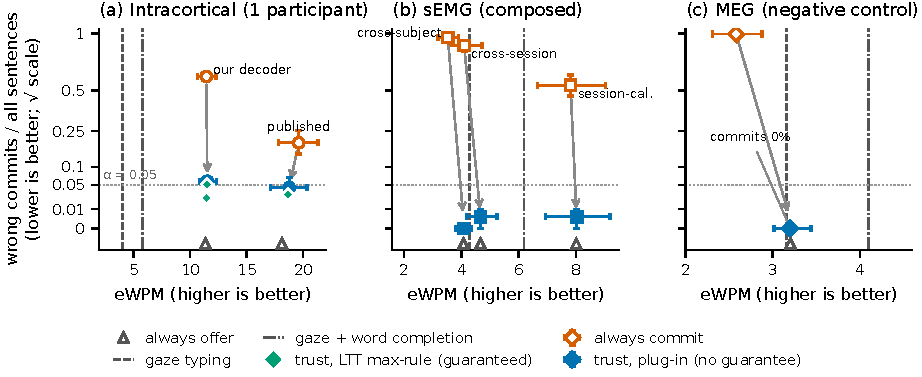
\includegraphics[width=\linewidth]{fig1_teaser.pdf}
  \caption{\textbf{The same trust layer removes almost all wrong commits on three device types.} Each panel plots the wrong-commit rate (share of sentences committed with an error) against effective words per minute (\ewpm{}) of a simulated user. Open markers: always commit the decoder's top sentence. Filled markers: the trust layer on the same decoder output; arrows connect the two. Dashed line: gaze typing alone (no BCI). Dotted line: target $\alpha = 0.05$. Error bars: 95\% bootstrap CIs over trials (a) and sentences (b, c; cluster bootstrap over the 17 unique sentences in c). (a)~Intracortical speech, Brain-to-Text '25, one participant, 816 test trials; ``our decoder'' is our phoneme-to-word decoder, ``published decoder'' is the published LM-rescored sentence. (b)~Forearm sEMG, 551 composed test sentences from 19 participants, three decoder conditions. (c)~MEG typing, 637 test instances (17 unique sentences) from 19 participants, our asynchronous M1-09 decoder.}
  \label{fig:teaser}
\end{figure}
